The authors plot graphs of percent of collisions against orbital radius, collision percent and residual collisions against impact parameters and impact velocity, and impact velocity and eccentricity against orbital radius and find that in the binary system, close to the binary, growth enabling events don't show any particular trend and any planets forming here seem to be results of "lucky" collisions from low speed encounters. But at a larger distance from the binary the growth resembles that of the single star system. 
\\
\begin{figure}[h] 
    \centering
    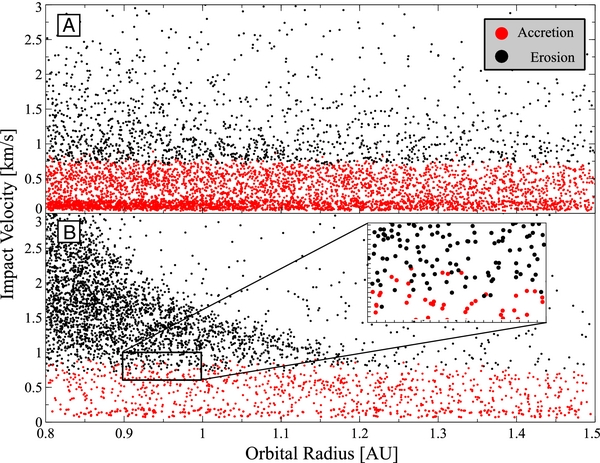
\includegraphics[height= 6cm , width= 8cm]{kepler34/apjl490718f4_lr.jpg}
    \caption{Spatial evolution of the impact velocity for each collision in the single star and circumbinary.}
    \label{12}
\end{figure}

\begin{figure}[h] 
    \centering
    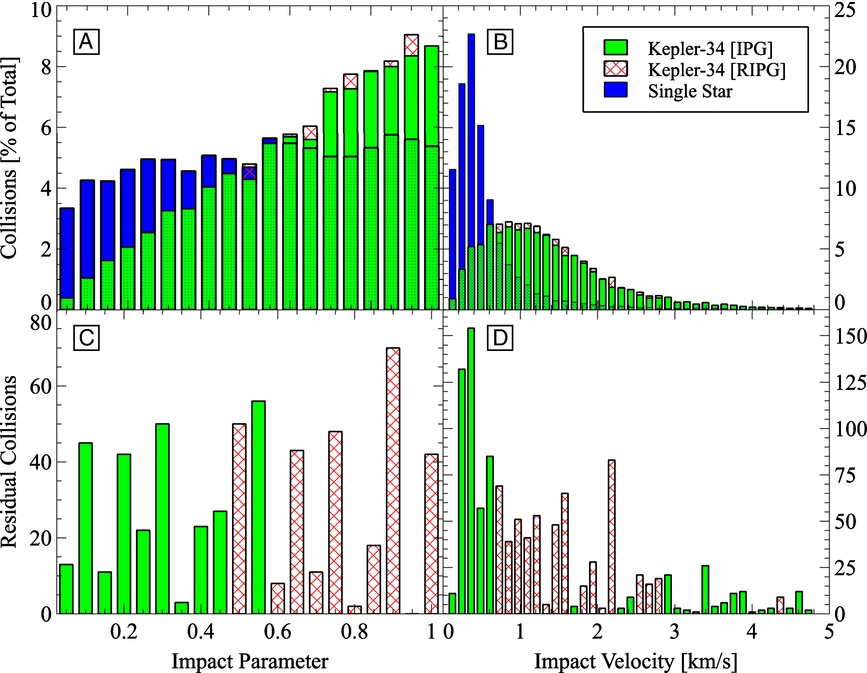
\includegraphics[height= 6cm , width= 8cm]{kepler34/apjl490718f3_hr.jpg}
    \caption{Distribution of impact parameter (A) and impact velocity (B) for each collision for the single star (blue) and circumbinary disk. The lower panels highlight the residual collision numbers between IPG (green) and RIPG (hashed).}
    \label{12}
\end{figure}
The simulation proves that the disk is a hostile environment for planetary growth and that only Kepler-47(AB)c could have formed in-situ while the rest must have formed at larger a where the protoplanetary disks were less perturbed by the binary stars and migrated inward to their current location.
